\subsubsection{Atividades}
Em SysML, uma atividade tem o propósito de descrever comportamento que transforma entradas em saídas, através de uma sequência de \textbf{ações}.

Ações são o bloco fundamental de descrição das atividades, mostrando como elas executam. Cada ação aceita entrada e produz saídas, que chamamos de \textbf{tokens}.

A saída de uma ação (token) se torna a entrada de outra, porque elas se conectam como peças, entrada em saída.

Fluxos de controle fornecem restrições adicionais sobre a maneira ou a ordem com que as ações que compõem uma atividade são executadas.

\subsubsection{Diagrama de Atividades}

O diagrama de atividades define as ações da atividade assim como o fluxo de entradas e saídas, e o controle entre elas. Assim, esse diagrama modela o comportamento de um caso de uso.

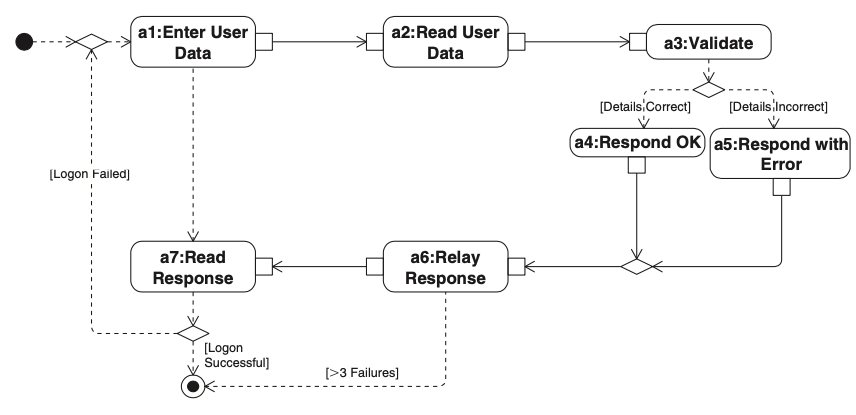
\includegraphics[width=\textwidth,height=\textheight,keepaspectratio]{figures/diagrama-atividades-1.png}